\subsection{Explicación formal del problema}
\label{subsec:problema3}
Sea el conjunto de puntos del primer cuadrante $C = \{(x_1, y_1), \hdots, (x_n, y_n)\}$. Se desea hallar alguna partición, $P$, del mismo que tenga cardinalidad mínima y cumpla la siguiente condición: $(\forall X \in P) (\exists r$ : semirrecta$) (\forall punto \in X)$ $punto \in r$. Esto es, que cada conjunto de la partición solo puede tener puntos que pertenecen a una misma semirrecta (sea cual sea esta). 
Notar que la segunda condición no restringe la posibilidad de que $r$ atraviese puntos de otro conjunto de la partición. 
%También ver que por la primer condición (cardinalidad mínima), si $r'$ es la semirrecta correspondiente a $X'$, no puede ocurrir que $r' \subset r$ pues en tal caso considero la partición $P'$, igual a $P$ salvo porque tengo $X'' = X \cup X'$ (que cumple la segunda condición dado que $r$ verifica bien) en lugar de $X$ y $X'$, y por tanto tiene cardinalidad estrictamente menor que $P$, lo que conduce a un absurdo. 

Por ejemplo, consideremos $C=\{(3,2), (3,5), (3,7), (5,6), (7,4)\}$. Tomemos la partición $P' = \{\{(3,2), (3,5)\}, \{(3,7)\}\},\{(5,6), (7,4)\}\}$. Para ver si $P'$ es solución de nuestro problema grafiquemos los puntos y trazemos una posible configuración de semirrectas correspondiente a la partición, como en la figura (\ref{fig:ej3-2})\footnote{En esta sección los gráficos usarán la siguiente convención: los puntos considerados están marcados con círculos y cuadrados, representando estos últimos el origen de las semirrectas. }. Viendo esto es claro que podría atravesarse todos los puntos con solo dos semirrectas en lugar de 3. Inspirados en la figura (\ref{fig:ej3-1}) deducimos que una solución es $P = \{\{(3,2), (3,5), (3,7)\},\{(5,6), (7,4)\}\}$. En este caso puntual además resulta que es la única solución posible (teniendo en cuenta que no nos importa el orden de los puntos por ser conjuntos). Aunque esto en general no vale, como se ve por ejemplo en las figuras (\ref{fig:ej3-3}) y (\ref{fig:ej3-4}), donde las elecciones de semirrectas inducen particiones claramente distintas.

\begin{figure}[H]
\centering
\begin{minipage}{0.49\textwidth}
  \centering
    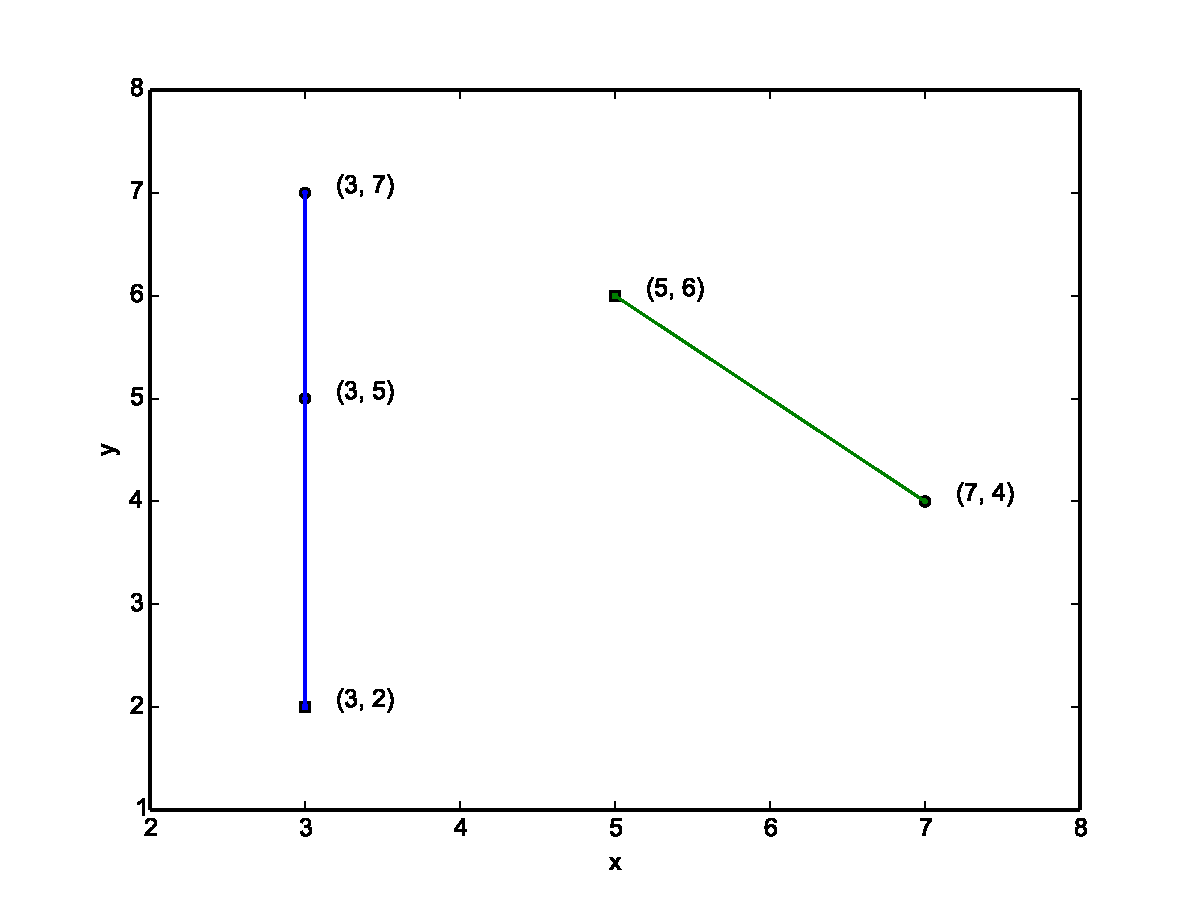
\includegraphics[width=1\textwidth]{img/ejemplos/ej3-1.pdf}
  \caption{\footnotesize Posible elección de semirrectas para la partición $P$.}
  \label{fig:ej3-1}
\end{minipage}%
\hspace{0.01\textwidth}
\begin{minipage}{0.49\textwidth}   
  \centering
    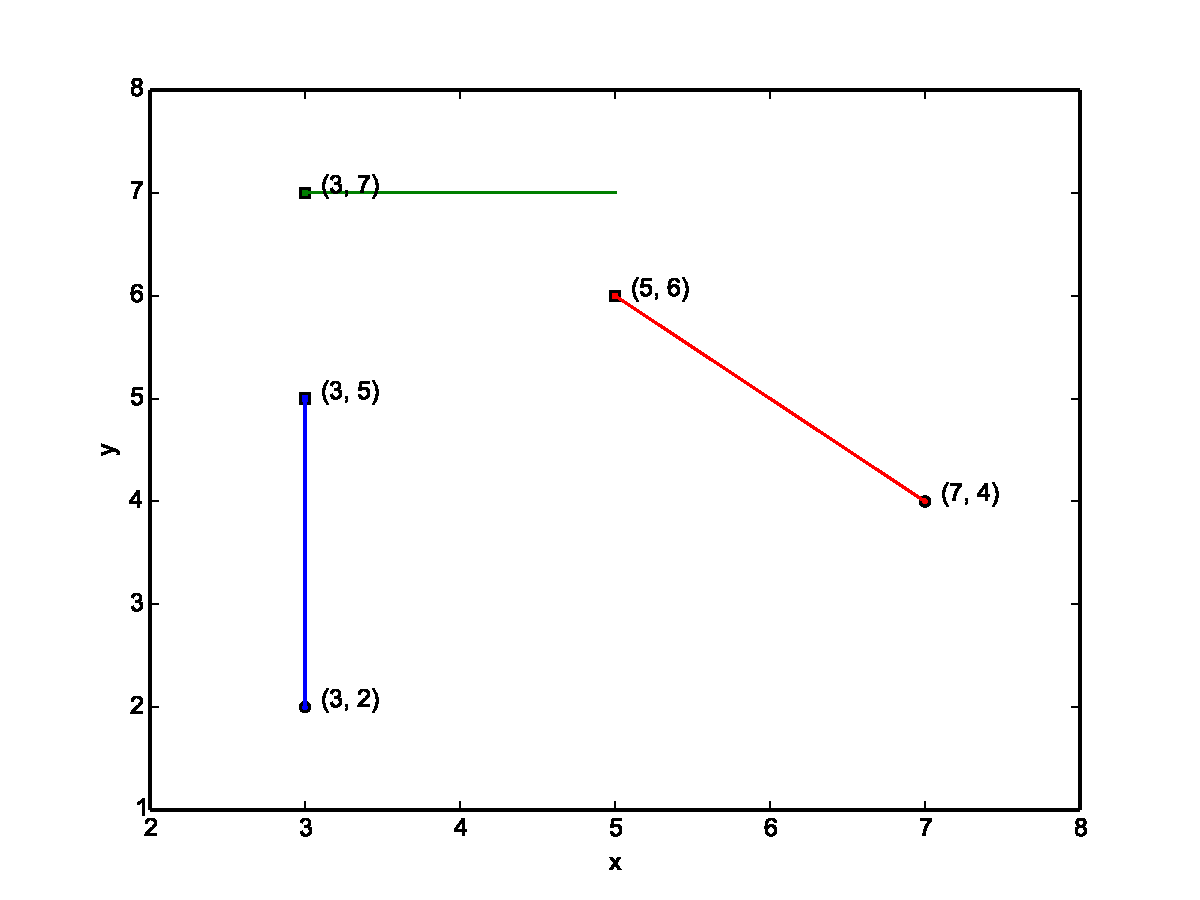
\includegraphics[width=1\textwidth]{img/ejemplos/ej3-2.pdf} 
  \caption{\footnotesize Posible elección de semirrectas para la partición $P'$.}
  \label{fig:ej3-2}
\end{minipage}%
\end{figure}

\begin{figure}[H]
  \centering
  \begin{minipage}{0.49\textwidth}
  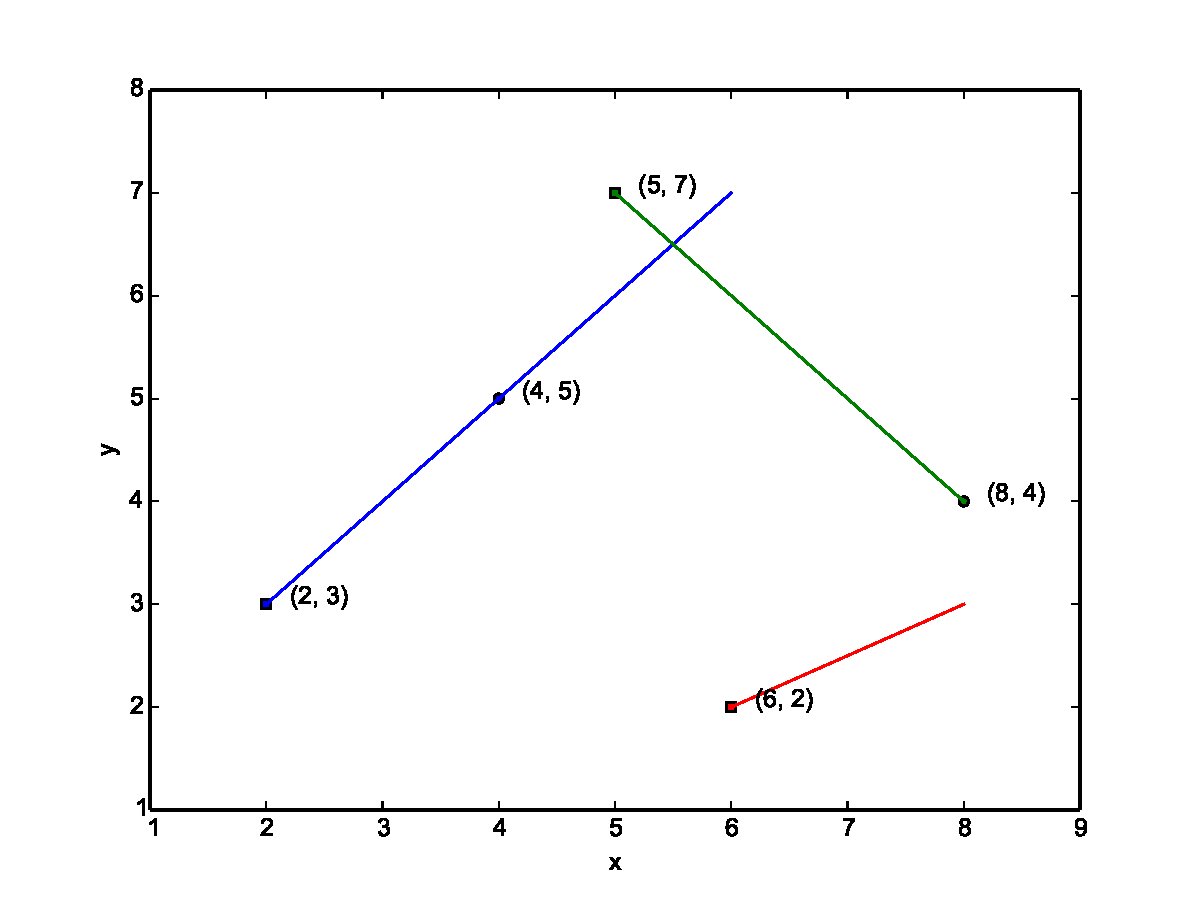
\includegraphics[width=0.75\textwidth]{img/ejemplos/ej3-3.pdf}
  \caption{\footnotesize Solución óptima para un conjunto dado de 5 puntos, donde no hay 3 puntos alineados.}
  \label{fig:ej3-3}
  \end{minipage}%
  \hspace{0.01\textwidth}
  \begin{minipage}{0.49\textwidth}
  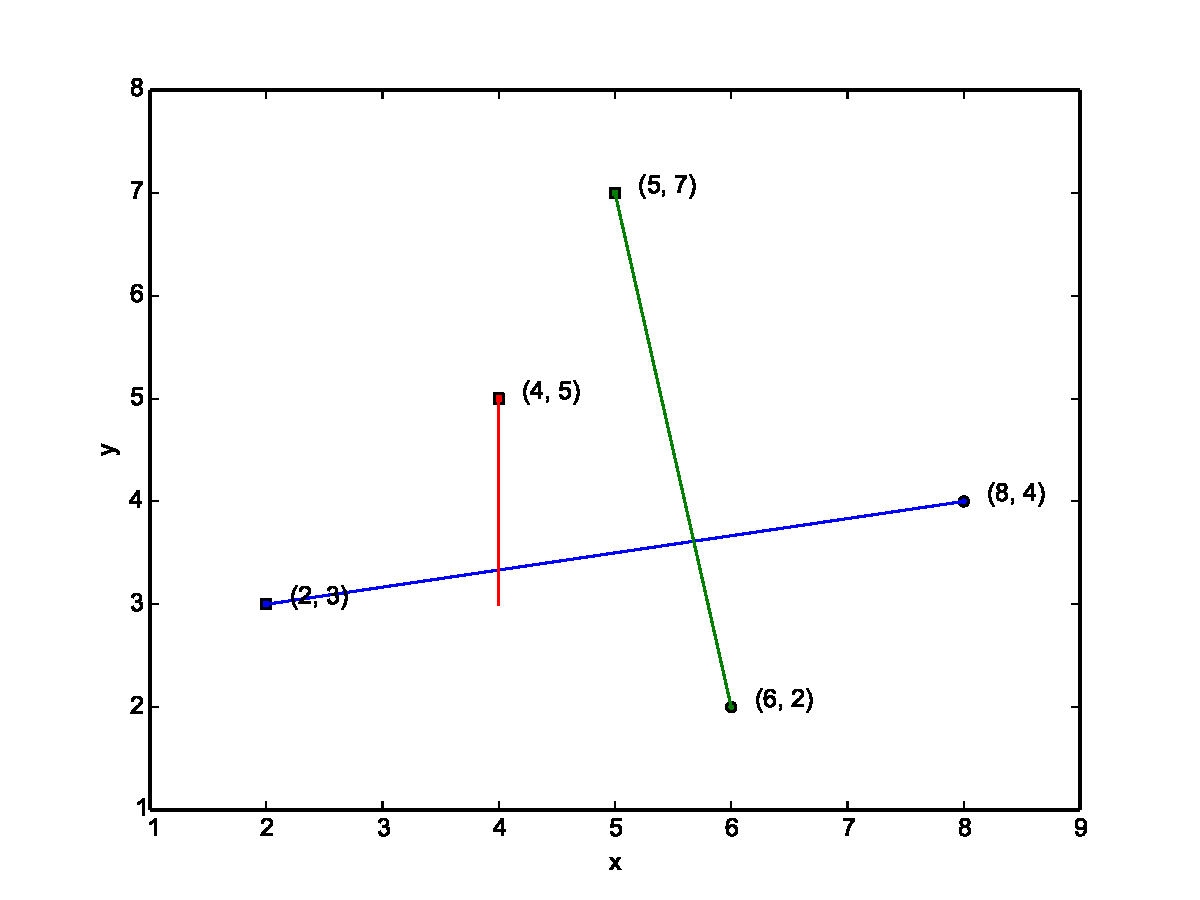
\includegraphics[width=0.75\textwidth]{img/ejemplos/ej3-4.pdf}
  \caption{\footnotesize Solución óptima para un conjunto dado de 5 puntos, donde no hay 3 puntos alineados.}
  \label{fig:ej3-4}
  \end{minipage}%
\end{figure}

Debido a que entre dos puntos siempre se puede establecer un semirrecta que los una, ningún conjunto de la partición solución, $P$, puede tener menos de dos elementos, salvo quizás uno (como ocurre en la figura \ref{fig:ej3-3})). Si tuviera al menos dos conjuntos en $P$ con un solo elemento, $X y X'$, entonces podría considerar $P'$, igual a $P$ salvo que tiene a $X'' = X \cup X'$ (que es válido porque seguro hay una semirrecta que una los dos puntos) y por lo tanto no posee a $X y X'$. Claramente el cardinal de $P'$ es estrictamente menor al de $P$, lo que es un absurdo pues $P$ era solución. Luego, $P$ puede tener a lo sumo un conjunto con un elemento.

Por lo dicho en el párrafo anterior, se puede establecer una cota superior al cardinal de la solución cuando tengo $n$ puntos: $\lceil\frac{n}{2}\rceil$ ¿Cuándo se alcanza dicha cota? Cuando no existe ninguna semirrecta que pueda atravesar más de dos puntos. Una disposición fácil de generar este tipo de casos es considerar $n$ puntos esparcidos sobre una circunferencia (una recta solo puede ser tangente o secante respecto a una circunferencia). En la figura (\ref{fig:ej3-5}) puede verse un ejemplo de esta situación para 16 puntos.

\begin{figure}[H]
  \centering
  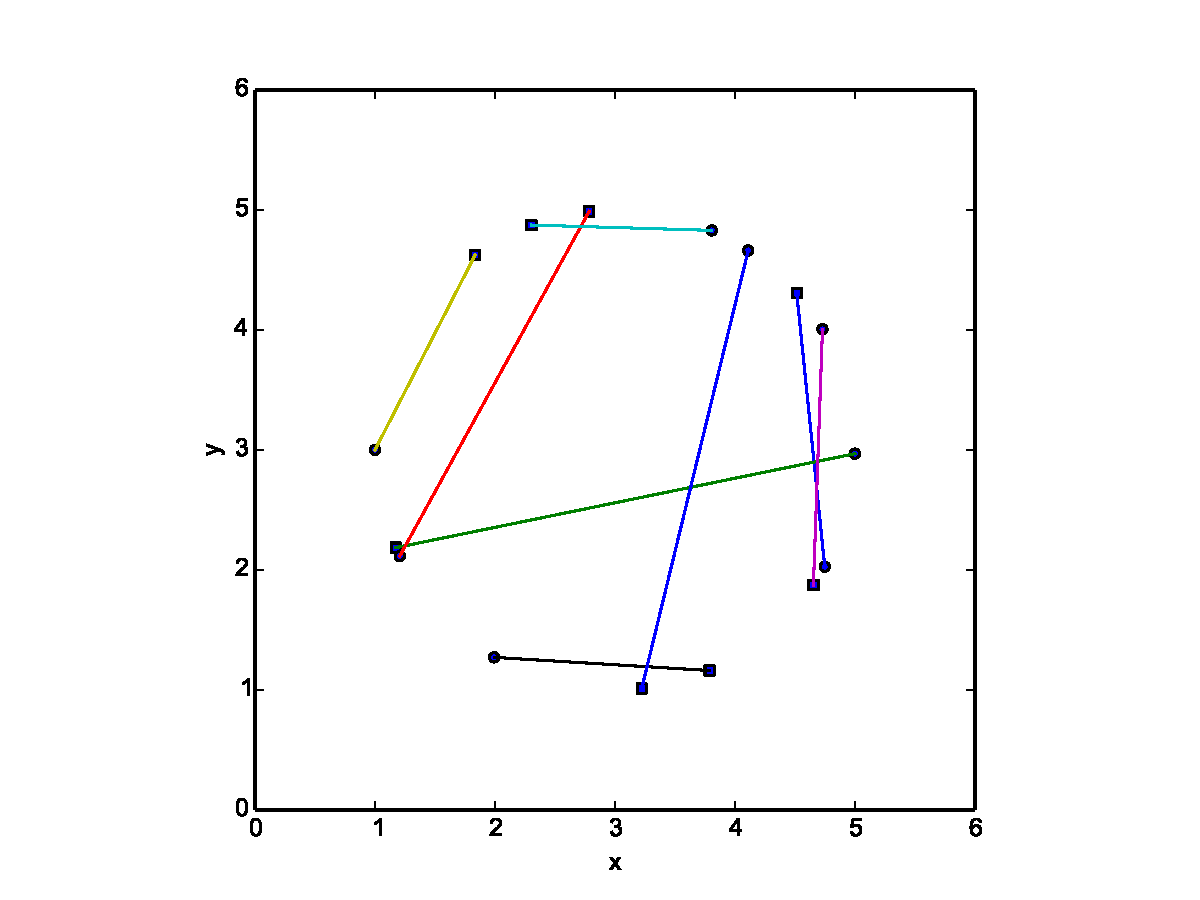
\includegraphics[width=0.70\textwidth]{img/ejemplos/ej3-5.pdf}
  \caption{\footnotesize Solución óptima para un conjunto de 16 puntos dispuestos sobre una circunferencia de radio 2 centrada en $(3,3)$.}
  \label{fig:ej3-5}
\end{figure}

\subsection{Explicación de la solución}
En esta sección daremos una breve explicación de porque el método de \texttt{backtracking} resulta correcto para resolver el problema presentado,  luego contaremos las podas y estrategias utilizadas, y finalmente presentaremos una explicación de las partes fundamentales de la implementación. 

\subsubsection{Árbol de posibilidades}
Los algoritmos de \texttt{backtracking} son un refinamiento de los algoritmos de fuerza bruta por lo que pensemos primero la solución usando este método. Este último tipo de algoritmos consisten en enumerar todos los posibles candidatos a solución del problema y ver si satisfacen las condiciones pedidas o no. En nuestro caso particular, todas los posibles candidatos van a ser las particiones que cumplan la segunda condición del enunciado, y de estas nos quedamos con alguna que tenga cardinal mínimo. 

El proceso de construir las particiones se puede pensar como un árbol en el que en cada nivel se agrega un nuevo conjunto de los posibles a la partición que estoy armando. Así, en el nivel 0 (la raíz) tengo un conjunto vacío. En el nivel 1 tengo todos los subconjuntos de $C$ que verifican que existe alguna semirrecta que los une. Al escoger alguno de estos conjuntos lo agregamos en la potencial partición. Debido a esto, en el nivel 2 tenemos un subconjunto de las posibilidades del nivel 1 estrictamente más pequeño pues debemos eliminar todas aquellas opciones que involucraban alguno de los puntos presentes en el conjunto previamente agregado (los conjuntos de la partición deben ser disjuntos). Se repite un procedimiento análogo hasta completar la partición, momento en el que estaremos parados en una hoja del árbol. 

Haciendo DFS (Depth-first search) recorremos todo el árbol de posibilidades, de forma que finalmente encontramos todas las particiones que cumplen la condición dos. Finalmente nos quedamos con alguna de cardinal mínimo (si hubiera más de una).

La correctitud de tal algoritmo es clara pues encuentra todo el universo de posibles soluciones, por lo que si efectivamente existe alguna eventualmente la obtiene. En particular, para todo conjunto finito es posible establecer particiones, así que siempre hay solución. 

La idea de \texttt{backtracking} es preservar esta garantía de correctitud pero agilizando la búsqueda mediante la utilización de podas en el árbol de posibilidades. Dicho de otra forma, un algoritmo de este tipo descarta \texttt{candidatos a soluciones parciales} que a partir de algún criterio podemos predecir que no nos van a conducir a la solución. En nuestro problema, un candidato a solución parcial es una partición en construcción. En la siguiente sección mostramos con que criterios los descartamos.

\subsubsection{Podas realizadas}
\begin{enumerate}
  \item Si actualmente estamos parados en un nodo de nivel $s$ (es decir que el cardinal de nuestro candidato a solución parcial es $s$) y anteriormente ya habíamos encontrado una solución en el nivel $s$, entonces no tiene sentido continuar por ese camino pues sabemos que todas los candidatos a soluciones a los que se arrive van a ser peores que un candidato previamente encontrado. De esta forma estamos ahorrándonos una búsqueda innecesaria y potencialmente muy costosa.
  \item Por lo observado en la sección \ref{subsec:problema3}, no tiene sentido considerar agregar conjuntos que tienen un solo elemento, salvo potencialmente en el último paso. Esto elimina muchas ramas del árbol.
\end{enumerate}

\subsubsection{Pseudocódigo}
  \begin{algorithm}[H]
  \begin{algorithmic}
  \caption{Pseudocódigo del procedimiento de \texttt{backtracking} en Kamehameha}
    \Procedure{backtracking}{Tablero $t$, int $step$}
    \If {$step \geq mejor$}
      \State $return$
    \EndIf
    \If {$t.Solucionado()$}
      \State $mejor \gets step$
      \State $mejor\_sol \gets t.Solucion()$
    \Else
      \For {$i \in [0,..., n),$ $t.EstaVivo?(i)$}
        \If {$t.SoloQuedaUno?()$}
          \State $t.Matar(i)$
          \State $backtracking(t, step+1)$
          \State $return$
        \EndIf
        \For {$j \in [0,..., n),$ $j \neq i \land t.EstaVivo?(j)$}
          \State $Tablero$ $sucesor \gets Copiar(t)$
          \State $Vector(int)$ $derrotados \gets [i, j]$ 
          \For {$k \in [0,..., n),$ $k \neq i \land k \neq j \land t.EstaVivo?(k)$}
            \If {$x_i \neq x_j \land y_i \neq y_j$}
              \If {$\frac{x_k-x_i}{x_j-x_i} = \frac{y_k-y_i}{y_j-y_i} \land MismoCuadrante?(i,j,k)$}
                \State $derrotados.AgregarAtras(k)$
              \EndIf
            \Else 
              \If {\small{$(AlinHor?(i,j,k) \lor AlinVer?(i,j,k)) \land MismoCuadrante?(i,j,k)$}}
                \State $derrotados.AgregarAtras(k)$
              \EndIf
            \EndIf
          \EndFor
          \State $sucesor.Matar(derrotados)$
          \State $backtracking(sucesor, step+1)$
        \EndFor
      \EndFor
    \EndIf
    \EndProcedure
  \end{algorithmic}
  \end{algorithm}

\subsection{Complejidad del algoritmo}

\subsection{Performance del algoritmo}